\section{Main evaluation}
\label{sec:evaluation}

We compare monitors on the OOD suite of Sinha et al.\ (Section~\ref{sec:background}) by Mean-OOD pAUROC@20 and by the cost of 1,000 evaluations.
The reasoning monitors are those of Sinha et al., with the scores and costs that they report.
We scored decision models and unadapted language models ourselves, from their binary logits or native probabilities, and price them at API or hosted prices.
We price Gleipnir at the cost of one B200 with one request at a time, at both rates of Section~\ref{sec:serving}, on the released serving stack.
Gleipnir 4B reads the compact instruction and Gleipnir 27B the full specification (Section~\ref{sec:training-setup}).
Figure~\ref{fig:frontier} shows the main comparisons. Table~\ref{tab:ood-all} in Appendix~\ref{app:ood-all} lists every monitor, together with its recall at a false-positive rate of 1\%, which is closer to deployment.

\begin{figure}[t]
\centering
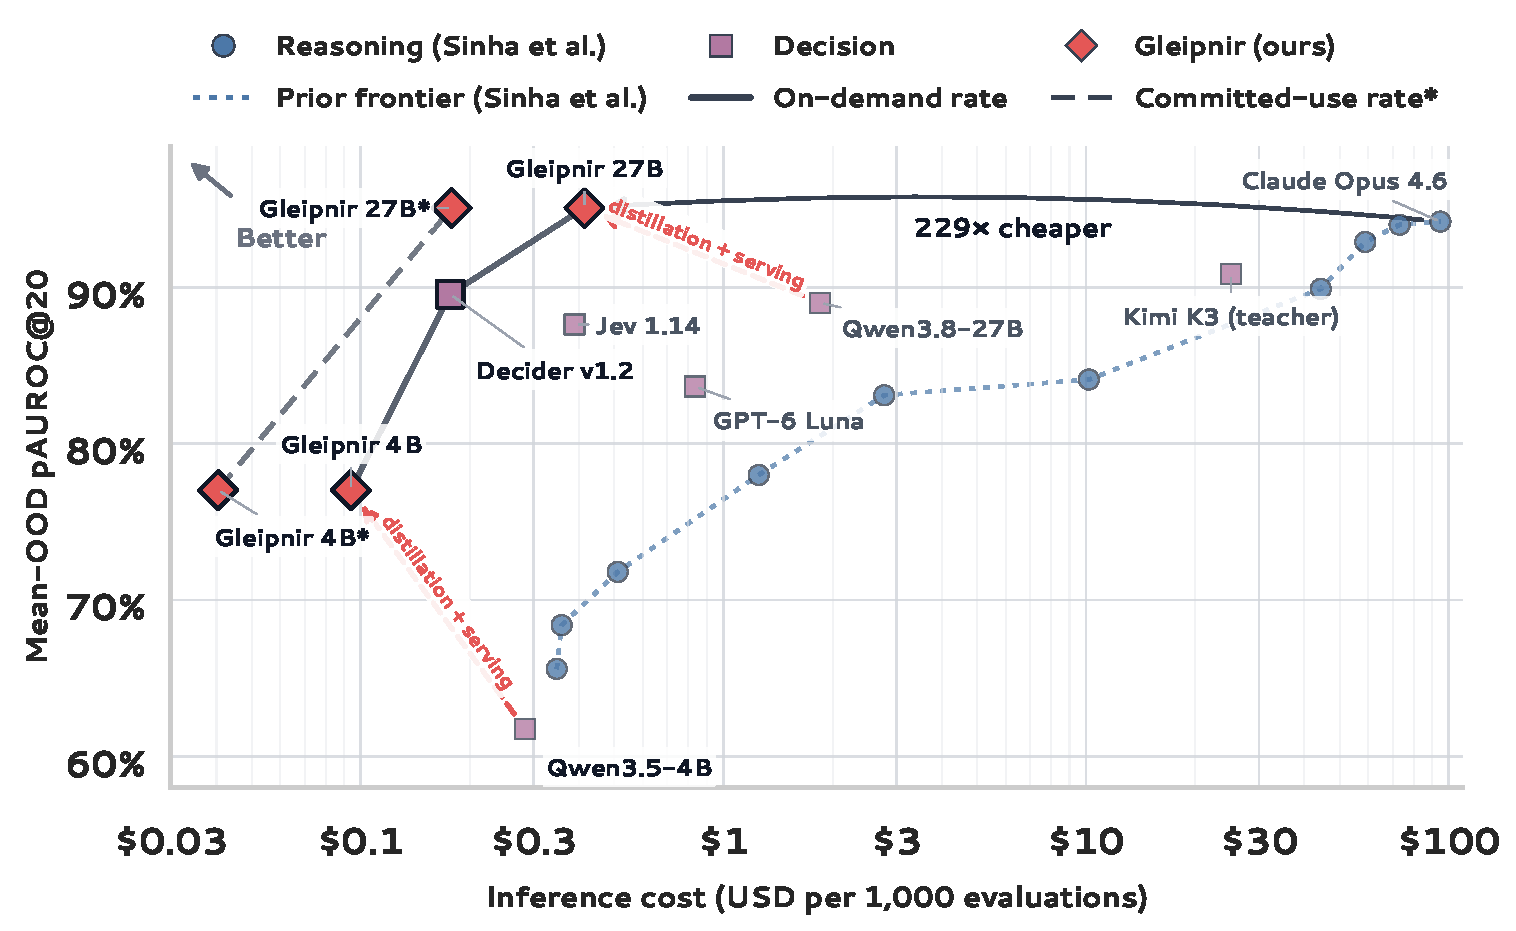
\includegraphics[width=\linewidth]{ood_frontier}
\caption{Gleipnir 27B matches the strongest reasoning monitor at 229 times lower cost on demand and 532 times lower with committed use. Mean-OOD pAUROC@20 against the inference cost per 1,000 evaluations (log scale). Reasoning monitors are those of \citet{sinha2026training} at their reported costs; we scored the decision models and unadapted language models at API or hosted prices. Gleipnir is priced at one B200 with one request at a time, at the on-demand rate (solid frontier) and at the committed-use rate (marked *, dashed frontier); each frontier treats costs within 3\% of each other as equal. Red arrows lead from each base model, at its hosted price, to the Gleipnir monitor distilled from it and served on our stack. For readability the figure omits further decision models, base models and reasoning monitors below the prior frontier; Table~\ref{tab:ood-all} lists them.}
\label{fig:frontier}
\end{figure}

\paragraph{Gleipnir 27B matches the strongest reasoning monitor at a fraction of its cost.}
It scores 0.951 Mean-OOD pAUROC@20 (95\% bootstrap interval 0.941--0.960) and Claude Opus 4.6, the strongest monitor of Sinha et al., scores 0.942.
The difference lies within the interval, while Gleipnir 27B costs 229 times less at the on-demand rate and 532 times less at the committed-use rate.
Its lead of 0.042 over its teacher, Kimi K3, comes from one task of SHADE-Arena (Appendix~\ref{app:shade}).

\paragraph{Training raises both base models, and Gleipnir 4B outperforms the recipe of Sinha et al.}
Training raises Qwen3.5-4B from 0.618 to 0.770 and Qwen3.8-27B from 0.890 to 0.951.
From the same base model, Gleipnir 4B scores 0.086 above the monitor that Sinha et al.\ train with SFT and RL.

\paragraph{At equal cost, Gleipnir 27B outperforms the strongest decision model.}
At the committed-use rate, Gleipnir 27B costs about the same as pplx-decider v1.2 (\$0.178 and \$0.176) and scores 0.055 higher in pAUROC@20.
At a false-positive rate of 1\%, it recalls 87.4\% of the harmful trajectories, 11.5 points more than pplx-decider v1.2 (Table~\ref{tab:ood-all}).

These results matter for deployment in two ways.
First, at these costs a deployment can check every trajectory, or every action, instead of a sample; Section~\ref{sec:serving-caching} prices the monitoring of every action.
Second, Claude Opus 4.6 lies within the bootstrap interval of Gleipnir 27B, close to the maximum, so the OOD suite no longer separates the strongest monitors; Section~\ref{sec:held-out} turns to harder benchmarks.
